\chapter{Event Summarization Challenge}
\label{cha:introduction}

% the code below specifies where the figures are stored
\ifpdf
    \graphicspath{{1_introduction/figures/PNG/}{1_introduction/figures/PDF/}{1_introduction/figures/}}
\else
    \graphicspath{{1_introduction/figures/EPS/}{1_introduction/figures/}}
\fi

\section{Motivation and Problem Statement}

A~very open definition of the word \emph{event}
given by WordNet~\cite{fellbaum1998wordnet,miller1995wordnet} is
\emph{``something that happens at a~given place and time''}.
Following this definition,
we are indeed surrounded by events,
most of which are of little to no interest for us.
A~concert somewhere in the world of a~band
that we do not even know may be a~good example.
For some events, however, we may care more, for example,
a~concert of a~band that we know and like,
even if it takes place at a~location far away from us.
Finally, for very few events, we may care a~lot,
maybe even enough to physically attend the event,
like a~concert of our favorite band
if it takes place in our city, is not sold out,
and not too expensive.

All this motivates the need for \emph{event summarization}.
If there is an event that we could not attend
for any given reason,
but that we are interested in,
a~good event summarization can help us get a~feeling
for the event's atmosphere.
Similarly, if there is an event that we attended,
we can revive the event's most fascinating moments
based on the event summarization.

A~\emph{media gallery} in the context of
our event summarization task is
a~\emph{best-of} compilation of photos, videos,
and microposts retrieved from social networks
that are related to a~given event.
Event summarization covers textual
as well as multimedia content.
We say a~media gallery is of high quality,
if it fulfills the following properties.

\begin{enumerate}
  \item \textit{Conciseness:}
        it conveys a~lot of information clearly
        and in few media items.
  \item \textit{Comprehensiveness:}
        it is complete and covers all representative
        elements or aspects of an event.
  \item \textit{Authenticity:}
        it is of undisputed origin and genuine.
  \item \textit{Diversity:}
        it shows a~great deal of variety.
  \item \textit{Interestingness:}
        it catches and holds the attention of the viewer.     
\end{enumerate}

\section{Research Question and Hypothesis}

The main research question for this thesis
can be formulated as follows.
 
\textit{``Can user-customizable
media galleries that summarize given events be
created solely based on textual and multimedia data
from social networks?''}

\noindent The hypothesis that we test in this thesis
can be formulated as follows.

We argue that through media galleries that leverage content
that was shared on social networks,
a~more \emph{authentic}, more \emph{concise},
more \emph{comprehensive}, more \emph{diverse},
and also more \emph{interesting}
view on events gets possible than by limiting oneself
to officially produced media content;
and that further such media galleries can be generated
more \emph{efficiently} and \emph{in shorter time}
than manually produced media galleries.

We validate these subjective and objective
criteria with experiments for events of different categories
such as sports, politics, culture, leisure,
music, conferences, \emph{etc.}

\section{Approach}

The objective of this thesis is the development
of methods for the automated summarization of events
based on media items shared on social networks.
A~schematic overview of the approach can be seen
in~\autoref{fig:thesis-diagram}.
As an event takes places and shortly thereafter
(symbolized by the timeline marked with \emph{2h Event}),
people share media items related to the event
on multiple social networks
(symbolized by the photo and video pictograms
above the event timeline).
Via the textual search APIs (Application Programming Interfaces)
of these different social networks,
we retrieve a~list of potentially event-relevant
microposts that either contain media items directly,
or that provide links to media items
on external media item hosting platforms.
Using third-party NLP tools,
we recognize and disambiguate named entities
in the microposts to predetermine their relevance.
We extract the binary media item data
from social networks or media item hosting platforms
and relate it to the originating microposts
(symbolized by the central cloud).
Using CBIR and CBVR techniques, we first deduplicate
exact-duplicate and near-duplicate media items,
and then cluster similar media items
(symbolized by the green, red, and orange markers).
We rank the deduplicated and clustered list
of media items and their related microposts
according to well-defined ranking criteria.
In order to generate interactive and user-customizable
media galleries that visually and audially summarize the
event in question, we compile the top-$n$ ranked
media items and microposts in an aesthetic way
(symbolized by the timeline marked with \emph{5min Summary}).

\begin{figure}[!ht]
  \centering
  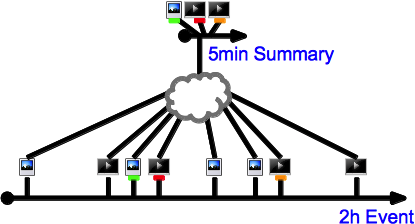
\includegraphics[]{thesis-diagram.png}
  \caption[Schematic depiction of event summary generation]
    {Schematic depiction of event summary generation
    based on deduplicated, clustered, and ranked media items
    for an exemplary event}
  \label{fig:thesis-diagram}
\end{figure}

\section{Contributions}

In this thesis, we report on methods for
the automated generation of event summaries.
This particular field of research touches on many related areas
of research and research communities,
amongst which social network research, multimedia content analysis,
Semantic Web and Natural Language Processing (NLP),
human factors in computing systems,
and Web services.
Early on in the process of this thesis,
we have sought and incorporated expert feedback based on
a~Doctoral Consortium paper~%
\cite{steiner2011enrichingunstructured}.
We have broken our contributions down into
the following topics.

\subsection{Social Network Multimedia and Data Analysis}

We have worked on methods for the aggregation, extraction,
deduplication, clustering, and compilation
of social media contents from
multiple social networks~%
\cite{rizzo2012whatfresh}.
Those methods were applied and evaluated
for the enhancement of conference experiences~%
\cite{khrouf2012aggregatingsocialmedia,khrouf2012confomaton}.

\subsection{Application of Semantic Web and NLP Techniques}

In order to make sense out of social network microposts,
we have worked on methods to consolidate and rank
the results of multiple named entity recognition and
disambiguation APIs and to track their data provenance~%
\cite{steiner2011addingmeaning}.
We have applied and evaluated those methods
for the consumer-oriented detection of trending microposts
on a~major commercial social network~%
\cite{steiner2011tweetconsumers}.


\subsection{Video Content and Metadata Analysis}

We have worked on methods for named entity extraction and
disambiguation for online videos based on closed captions
and other textual metadata, which make online video
more accessible, searchable, and interconnected~%
\cite{steiner2010semwebvid,steiner2010semwebvidchallenge}.
Further, we have combined those textual methods with 
video content analysis methods for the on-the-fly detection
of shot boundaries for online videos~%
\cite{steiner2012shotdetection}.
We have defined aesthetic principles
for the automated generation of media gallery layouts
for visual and audial event summarization
based on social network multimedia data~%
\cite{steiner2012definingaesthetic}.
        
\subsection{Crowdsourcing}

The video content analysis methods mentioned before
were combined with methods for the crowdsourced detection
of events in online videos~%
\cite{steiner2011crowdsourcingevent}.
We have further worked on crowdsourcing methods
for the extraction of knowledge items from arbitrary Web pages~%
\cite{steiner2012sekiathome,steiner2012sekiathomechallenge}.

\subsection{Studies}

We have contributed an examination of Linked Data usage and
visualization techniques of a~major commercial search engine~%
\cite{steiner2010howgoogleisusing}.
In addition to that, we have studied the usefulness and relevance
of social network updates which were added to search engine
results pages (SERP) of a~major commercial search engine~%
\cite{steiner2012addingrealtime}.

\subsection{Multimodal Search Engines}

We have worked on an examination of context-aware querying
for multimodal search engines~%
\cite{etzold2012contextawarequerying,steiner2012isearch}.
Further, we have studied user interface constraints on
mobile and desktop devices for a~multimodal search engine
and demonstrated that those constraints can be overcome~%
\cite{steiner2012onesizedoesnotfitall}.


\subsection{Web Service Description}

We have worked on methods for the semantic description of Web APIs,
their discoverability, their automated consumption,
their semantic interlinking, and their social aspects~%
\cite{verborgh2011descriptionandinteraction,verborgh2011efficientruntime,verborgh2011integratingdata,verborgh2012capturingthefunctionality,verborgh2012functionalcomposition,verborgh2012functionaldescriptions,verborgh2012missinglinks,verborgh2012restdesc,verborgh2012socialdescriptionrevolution}.
We have studied the feasibility of truly RESTful behavior
for Web APIs in the sense of Dr. Roy Fielding~%
\cite{steiner2011fulfilling}.
        
\subsection{Standardization and Specifications}        
We have helped to shape a~W3C specification on media
fragment addressing schemes for audio and video items~%
\cite{troncy2012mediafragments}.
Further, we have worked on the definition of a~unified framework
for the description of multimedia content objects~%
\cite{axenopoulos2012isearch,daras2011unifiedframework}.
Finally, we have contributed to a~white paper on the
Future Media Internet Architecture~%
\cite{alduan2011futureinternet}.

\subsection{Others}

We have developed methods for unobtrusively fixing
common annoyances on arbitrary Web pages~%
\cite{steiner2012xkcd37}.

\section{Thesis Structure}

Each chapter is closed by a~final section called
\emph{Chapter Notes}, which contains references to the publications
that the chapter is based upon
and in some cases pointers to related material for further reading.
The remainder of this thesis is structured as follows. 

\paragraph{\autoref{cha:background}:}

This chapter introduces the Semantic Web and its technologies.
Starting from the non-semantic Web,
we show how structured data can be added to Web pages
and briefly present DBpedia as a~knowledge base
founded on structured data extracted from Wikipedia.
We then continue with the Resource Description Framework
and explain how it represents facts with triples.
We provide examples of RDF's different serialization formats.
Afterwards, we outline the Semantic Web vision of
a~global giant database and present the Semantic Web
query language SPARQL.
We close the chapter with an introduction of Sir Tim Berners-Lee's
Linked Data principles and show how data publisher that publish
datasets according to those principles are visualized in the
Linking Open Data cloud.

\paragraph{\autoref{cha:social-networks}:}

This chapter provides the necessary definitions and terms
that we will use throughout this thesis. 
It introduces social networks and media platforms as concepts
\emph{per~se} and then lists the most popular social networks
together with their core features and multimedia data support.
We briefly look at decentralized social networks and explain
why we do not consider them in this thesis.
Finally, we propose a~classification scheme for social networks
that classifies them by their level of media item support.

\paragraph{\autoref{cha:micropost-annotation}:}

In this chapter, we describe how microposts can be semantically annotated
in order to make sense of their contents.
We show how we have developed two browser extensions to obtain access
to real-world micropost data of actual micropost consumers.
In continuation, we show how Natural Language Processing (NLP)
Web services, machine translation, and part-of-speech tagging (POS)
are combined by our annotation workflow
and how the results of multiple NLP services are consolidated and reconciled.
We show how provenance information can be automatically added
to the generated output, so that the contribution
of each Web service to the combined result is traceable,
which is desirable to acknowledge and credit each service's work 
and also for debugging purposes.

\paragraph{\autoref{cha:eventdetection}:}

This chapter is about breaking news event detection 
based on concurrent Wikipedia edits.
We have developed an application that automatically
reports breaking news event candidates by clustering 
articles from multi-language editing activity streams
and checking if well-defined breaking news conditions are fulfilled.
The application uses social networks for plausibility checks
in order to avoid false-positive alerts,
\emph{i.e.}, a~breaking news event has to be reflected on Wikipedia
\emph{and} on social networks.
We evaluate the event detection system with various
global and local news events for its timeliness and accuracy.

\paragraph{\autoref{cha:media-item-extraction}:}

In this chapter, we describe how media items can be extracted
from different social networks.
We introduce an alignment scheme that acts as an abstraction layer
to overcome the underlying differences in data structure of 
the supported social networks.
We evaluate the media item extractors with nine different events
and motivate the need for media item deduplication and ranking.

\paragraph{\autoref{cha:shot-boundary-detection}:}

In this chapter, we present an algorithm and an 
accompanying application for the task of detecting
camera shot boundaries on-the-fly in streaming Web video,
which is a~required step for the deduplication of videos
and photos contained in videos.
We evaluate the approach with videos from a~popular video hosting platform in form of a~browser extension.

\paragraph{\autoref{cha:media-item-deduplication}:}

This chapter is about the on-the-fly deduplication and clustering
of media items extracted from social networks.
We analyze reasons for the occurrence of exact-duplicate
and near-duplicate media items and introduce an algorithm
tailored to this task, incorporating matching conditions
that are based on the findings of the analysis.
We evaluate the algorithm with two events
and show its effectiveness.

\paragraph{\autoref{cha:media-item-ranking}:}

In this chapter, we focus on ranking media item clusters
that contain visually similar media items.
We show how social interactions from different social networks
can be merged in order to obtain a~network-agnostic view
on the performance of the clustered media items.
Further, we show an algorithm for the selection of
one representative media item per cluster that represents
all media items contained in the same cluster.
We then propose a~ranking formula that is based on both
social interactions and other features.
We evaluate our ranking formula by comparing the ranked results
for a~given event with event highlight summaries regarding the same event
that were created by different social networks.

\paragraph{\autoref{cha:media-item-compilation}:}
\paragraph{\autoref{cha:future-work}:}

\bibliographystyle{plainnat}
\clearpage
\bibliography{backmatter/references}
